\documentclass[conference]{IEEEtran}

\usepackage{cite}
\usepackage{amsfonts,amsmath,amssymb,amsthm,booktabs,color,enumitem,graphicx}


% correct bad hyphenation here
\hyphenation{op-tical net-works semi-conduc-tor}


\begin{document}

\title{Deployment pipeline}

\author{\IEEEauthorblockN{Olli Rissanen}
\IEEEauthorblockA{Department of Computer Science\\
University of Helsinki\\
Helsinki, Finland\\
Email: olli.rissanen@helsinki.fi}}

% make the title area
\maketitle


\begin{abstract}
Currently more and more software companies are moving to lean practices, which often include shorter delivery cycles and thus shorter feedback loops. However, to achieve continuous customer feedback and to eliminate work that doesn't generate value, even shorter cycles are required. In continuous deployment the software functionality is deployed continuously at customer environment. This process includes both automated builds and automated testing, but also automated deployment. This adds more elements to the development pipeline, which often in a lean team consists of a version control system and a continuous integration server. Automating the whole process minimizes the time required for implementing new features in software, and allows for faster customer feedback. However, adopting continuous deployment doesn't necessarily mean that more value is created for the customer. 

According to multiple authors,  
\end{abstract}
% IEEEtran.cls defaults to using nonbold math in the Abstract.
% This preserves the distinction between vectors and scalars. However,
% if the conference you are submitting to favors bold math in the abstract,
% then you can use LaTeX's standard command \boldmath at the very start
% of the abstract to achieve this. Many IEEE journals/conferences frown on
% math in the abstract anyway.

% no keywords




% For peer review papers, you can put extra information on the cover
% page as needed:
% \ifCLASSOPTIONpeerreview
% \begin{center} \bfseries EDICS Category: 3-BBND \end{center}
% \fi
%
% For peerreview papers, this IEEEtran command inserts a page break and


% creates the second title. It will be ignored for other modes.
\IEEEpeerreviewmaketitle

%Perusteet

%Kiinnostava
%Innostava
%Tehtävissä

%Määrittele
% Tutkimusongelma, siis mitä haluat ymmärtää tai selvittää
% Tavoitteet
% Menetelmät
% Rajaus

%Mahdollisia toteutustapoja
% Vertaile kahta tai useampaa lähestymistapaa
% Etsi empiiristä todistusaineistoa jonkin väitteen puolesta tai sitä vastaan
% Kuvaa tapausyrityksen tilanne ja vertaile kirjallisuuteen
%

%Haasteet

%In fact, one sign of a good application architecture is that it allows the application
%to be run without much trouble on a development machine.

\section{Introduction} %why is this problem interesting?
Continuous deployment is an extension to continuous integration, where the software functionality is deployed frequently at customer environment. While continuous integration defines a process where the work is automatically built, tested and frequently integrated to mainline \cite{fowler2006continuous}, often multiple times a day, continuous deployment adds automated acceptance testing and deployment. The purpose of continuous deployment is that as the deployment process is completely automated, it reduces human error, documents required for the build and increases confidence that the build works \cite{cdbook}. %Explain pipeline here

In an agile process software release is done in periodic intervals \cite{cockburn2002agile}. Compared to waterfall model it introduces multiple releases throughout the development. Continuous deployment, on the other hand, attemps to keep the software ready for release at all times during development process \cite{cdbook}. Instead of stopping the development process and creating a build as in an agile process, the software is continuously deployed to customer environment. This doesn't mean that the development cycles in continuous deployment are shorter, but that the development is done in a way that makes the software always ready for release.

It should also be made clear that continuous delivery differs from continous deployment. Refer to Fig. \ref{fig1} for a visual representation of differences in continuous integration, delivery and deployment. Both include automated deployment to a staging environment. Continuous deployment includes deployment to a production environment, while in continuous delivery the deployment to a production environment is done manually. The purpose of continuous delivery is to prove that every build is proven deployable \cite{cdbook}. While it necessarily doesn't mean that teams release often, keeping the software in a state where a release can be made instantly is often seen beneficial.

Adopting a continuous deployment process doesn't necessarily mean that more value is delivered to a customer. Avinash Kaushik states in his Experimentation and Testing primer \cite{kaushik} that "80\% of the time you/we are wrong about what a customer wants". Mike Moran also found similar results in his book Do It Wrong Quickly, stating that Netflix considers 90\% of what they try to be wrong. A way to tackle this issue is to adopt a process of continuous experimentation, where the entire R&D system responds and acts based on instant customer feedback, and where actual deployment of software functionality is seen as a way of experimenting and testing what the customer needs \cite{olsson2012climbing}.

%Mitä continous experimentation tekee?

Continuous experimentation requires operational changes to the deployment pipeline. 

\begin{figure}[!t]
	\centering
	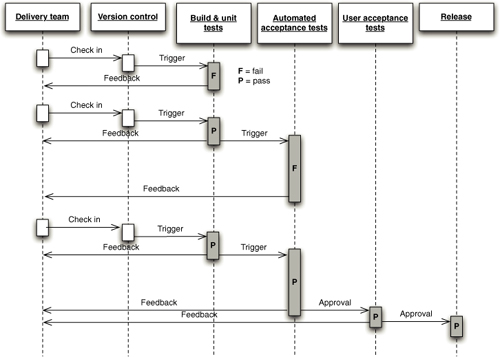
\includegraphics[width=3.5in]{developmentprocess.jpg}
	\caption{Architecture of the development process \cite{cdbook}.}
	\label{fig1}
\end{figure}


\section{Methods} %how did I find the papers?


\section{Results} %Pure analysis on the papers

\section{Discussion} %Own speculation


\section{Conclusion} %Short wrap-up. Contains the key points


\bibliography{IEEEabrv,references}{}
\bibliographystyle{IEEEtran}
% trigger a \newpage just before the given reference
% number - used to balance the columns on the last page
% adjust value as needed - may need to be readjusted if
% the document is modified later
%\IEEEtriggeratref{8}
% The "triggered" command can be changed if desired:
%\IEEEtriggercmd{\enlargethispage{-5in}}

% references section

% can use a bibliography generated by BibTeX as a .bbl file
% BibTeX documentation can be easily obtained at:
% http://www.ctan.org/tex-archive/biblio/bibtex/contrib/doc/
% The IEEEtran BibTeX style support page is at:
% http://www.michaelshell.org/tex/ieeetran/bibtex/

% argument is your BibTeX string definitions and bibliography database(s)
%\bibliography{IEEEabrv,../bib/paper}
%
% <OR> manually copy in the resultant .bbl file
% set second argument of \begin to the number of references
% (used to reserve space for the reference number labels box)
%\begin{thebibliography}{1}

%\bibitem{IEEEhowto:kopka}
%H.~Kopka and P.~W. Daly, \emph{A Guide to \LaTeX}, 3rd~ed.\hskip 1em plus
%  0.5em minus 0.4em\relax Harlow, England: Addison-Wesley, 1999.

%\end{thebibliography}




% that's all folks
\end{document}


